\usepackage{amsthm}

\newtheorem{theorem}{Theorem}[chapter]
\newtheorem{lemma}           [theorem] {Lemma}   
\newtheorem{folg}           [theorem] {Folgerung}   

\newtheorem{frage}       [theorem] {Frage}   
\newtheorem{question}       [theorem] {Question}   
\newtheorem{aufgabe}       [theorem] {Aufgabe}   
\newtheorem{exercise}       [theorem] {Exercise}  

\newtheorem{proposition}     [theorem] {Proposition}  
\newtheorem{satz}     [theorem] {Satz}  
\newtheorem{fact}{Fact}
\newtheorem{definition}      [theorem] {Definition} 

\theoremstyle{definition} 
\newtheorem{bemerkung}     [theorem] {Bemerkung}  
\newtheorem{beispiel}       [theorem] {Beispiel}  
\newtheorem{example}       [theorem] {Example}  
\newtheorem*{example*} {Example}  
\newtheorem{notation}       [theorem] {Notation}  
\newtheorem*{Faust}[theorem]{Rule of Thumb}
\newtheorem*{Boxx}[theorem]{Concept}

Next we define the notions of convergence and limits:
\begin{Definition}[Convergence/divergence of sequences]\label{def:convlim}
    Let $(a_n)_{n\in\mathbb{N}}$ be a~sequence in $\mathbb{K}$. We say that
\begin{itemize}
 \item[--] $(a_n)_{n\in\mathbb{N}}$ is \emph{convergent to $a\in \mathbb{K}$} if for all $\varepsilon>0$ there exists some $N=N(\varepsilon)\in\mathbb{N}$ such that for all $n\geq N$ holds $|a_n-a|<\varepsilon$. In this case, we write
\[\lim_{n\to\infty}a_n=a.\]
 \item[--] $(a_n)_{n\in\mathbb{N}}$ is \emph{divergent} if it is not convergent, i.e., for all $a\in \mathbb{K}$ holds: There exists some $\varepsilon>0$ such that for all $N$ there exists some $n>N$ with $|a_n-a|\geq\varepsilon$.
\end{itemize}

\end{Definition}

Convergence for real sequences means that if you give any small distance $\varepsilon$, one
finds that all sequence members $a_n$ lie in the interval $(a-\varepsilon, a+\varepsilon)$ with the exception of only \emph{finitely} many.

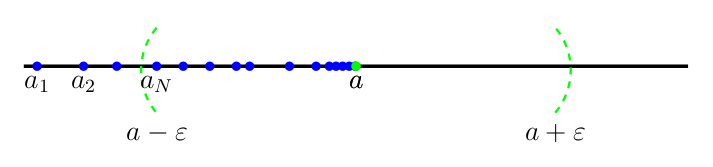
\includegraphics{./conv.png}

\begin{example}
\begin{itemize}
	\item Show: $(a_{n})_{n \in \mathbb{N}}$ with $a_n = (1/n)$ is convergent with limit $0$.
	\item Show: $(b_{n})_{n \in \mathbb{N}}$ with $b_n = (1/\sqrt{n})$ is convergent with limit $0$.
		\begin{proof}
			Let $\varepsilon > 0$. Choose $N > \frac{1}{\varepsilon^2}$. Then for all $n \geq N$, we have
				$$
					|b_n - 0| = \frac{1}{\sqrt{n}} \leq \frac{1}{\sqrt{N}} < \varepsilon 
				$$
			This means $b_n$ is arbitrarily close to $0$, eventually.
		\end{proof}
	\item Show: $(d_{n})_{n \in \mathbb{N}}$ with $\displaystyle d_n = \frac{1}{\sqrt{1 + \frac{1}{n}}}$ is convergent with limit $1$.
			\begin{proof}
			We know that $\sqrt{1 + 1/n}$ is always greater than $1$. Therefore, we can calculate:
				$$
				|1 - \frac{1}{\sqrt{1 + \frac{1}{n}}} |^2  \leq 
				\frac{ 1- 2 \sqrt{1 + \frac{1}{n}} + 1 + \frac{1}{n}}{1 + \frac{1}{n}} 
				$$
				$$
				\leq		\frac{ 1- 2 + 1 + \frac{1}{n}}{1 + \frac{1}{n}}		= 	
				\frac{ \frac{1}{n}}{1 + \frac{1}{n}} \leq \frac{1}{n}
				$$
			The square root is a monotonically increasing function, and hence, we can put the square root to both
			sides and get the inequality:
				$$
					0 ~\leq~ 1 - \frac{1}{\sqrt{1 + \frac{1}{n}}} ~\leq~ \frac{1}{\sqrt{n}}
				$$
			By the sandwich theorem of Homework 1, this shows that the sequence $(e_n)_{n \in \mathbb{N}N}$ given by
			$e_n := 1 - \frac{1}{\sqrt{1 + \frac{1}{n}}}$ is convergent with limit $0$. Then we use
			the limit theorem to get:
				$$
					\lim_{n \rightarrow \infty} d_n = \lim_{n \rightarrow \infty} (1 - e_n) = 
					\lim_{n \rightarrow \infty} 1 - \lim_{n \rightarrow \infty} e_n = 1 - 0 = 1
				$$
		\end{proof}
\end{itemize}
\end{example}


\begin{Remark}{}
\begin{enumerate}[(a)]
\item It can be shown that for a~complex sequence $(a_n)_{n\in\mathbb{N}}$, convergence to $a\in\mathbb{C}$ holds true if, and only if, $(\Re(a_n))_{n\in\mathbb{N}}$ converges to $\Re(a)$ \underline{and} $(\Im(a_n))_{n\in\mathbb{N}}$ converges to $\Im(a)$
\item In fact, convergence can also be defined for sequences in some arbitrary normed vector space $V$ (for the definition of a~normed space, e.g.\ consult the linear algebra script). Then one has to replace the absolute value by the norm (e.g., ``$\|a_n-a\|<\varepsilon$''.)
\item Due to the fact that for any $N\in\mathbb{N}$, we can find some $x\in\mathbb{R}$ with $x>N$, we can equivalently reformulate the convergence definition as follows:
``$(a_n)_{n\in\mathbb{N}}$ is convergent to $a\in \mathbb{R}$ if for all $\varepsilon>0$ there exists some $N=N(\varepsilon)\in\mathbb{R}$ such that for all $n\geq N$ holds $|a_n-a|<\varepsilon$''. In the following, we just write ``there exists some $N$''.
\end{enumerate}
\end{Remark}

What does convergence mean?

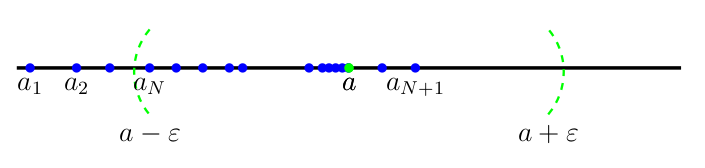
\includegraphics{./conv2.png}

Outside any $\varepsilon$-neighbourhood of $a$ only finitely many elements of the sequence exist.

\begin{example}\label{ex:basicconvseq}
 \begin{enumerate}[(a)]
  \item The real sequence $(\frac1n)_{n\in\mathbb{N}}$ converges to 0.\\
{\em Proof:} Let $\varepsilon>0$ (be arbitrary): Choose $N=\frac1\varepsilon+1=\frac{1+\varepsilon}\varepsilon$.\\
Then for all $n\geq N$ holds
\[\frac1n\leq\frac1N=\frac{\varepsilon}{1+\varepsilon}<\varepsilon.\]
Therefore
\[\left|\frac1n-0\right|=\frac1n<\varepsilon.\]
	\whiteskipsmall
\item  The real sequence $((-1)^n)_{n\in\mathbb{N}}$ is divergent.\\
{\em Proof by contradiction:}\\
Assume that $((-1)^n)_{n\in\mathbb{N}}$ is convergent to $a\in\mathbb{R}$. Then take e.g.\ $\varepsilon=\frac1{10}$. Due to convergence, we should have some $N$ such that for all $n\geq N$ holds
\[|(-1)^n-a|<{\textstyle\frac1{10}}.\]
Thus we have that $|-1-a|<\frac1{10}$ and $|1-a|<\frac1{10}$. As a~consequence,
\[2=|1+a-a+1|\leq|1+a|+|-a+1|=|1+a|+|a-1|<{\textstyle\frac1{10}+\frac1{10}=\frac1{5}}.\]
This is a contradiction.\hfill$\Box$
\item For $q\in\mathbb{C}\backslash\{0\}$ with $|q|<1$ the complex sequence $(q^n)_{n\in\mathbb{N}}$ converges to 0.\\
{\em Proof:}
$|q|<1$ gives rise to $\frac1{|q|}>1$, whence $\frac1{|q|}-1>0$. Therefore, we are able to apply Bernoulli's inequality (see tutorial) in the following way:

\[\frac1{|q|^n}=\left(1+\left(\frac1{|q|}-1\right)\right)^n
=\left(1+\left(\frac{1-|q|}{|q|}\right)\right)^n\geq 1+n\cdot \left(\frac{1-|q|}{|q|}\right),
\]
and thus
\[|q|^n\leq \frac1{1+n\cdot \left(\frac{1-|q|}{|q|}\right)}=\frac{|q|}{|q|+n\cdot ({1-|q|})}.\]
Now let $\varepsilon>0$ (be arbitrary):

Choose
\[N=\frac{|q|}{\varepsilon\cdot(1-|q|)}-\frac{|q|}{1-|q|}+1\]
Then for all $n\geq N$ holds
\[n>\frac{|q|}{\varepsilon\cdot(1-|q|)}-\frac{|q|}{1-|q|}\]
and thus
\[n\cdot ({1-|q|})>\frac{|q|}{\varepsilon}-|q|.\]
This leads to
\[|q|+n\cdot ({1-|q|})>\frac{|q|}{\varepsilon},\]
whence
\[\frac{|q|}{|q|+n\cdot ({1-|q|})}<\varepsilon.\]
The above calculations now imply
\[|q^n-0|=|q|^n\leq\frac{|q|}{|q|+n\cdot ({1-|q|})}<\varepsilon.\]
\hfill$\Box$
 \end{enumerate}
\end{example}

\begin{Remark}{}
The choice of the $N$ often seems ``to appear from nowhere''. However, there is a~systematic way to formulate the proof. For instance in a), we need to end up with the equation $|\frac1n-0|<\varepsilon$ or, equivalently, $\frac1n<\varepsilon$. Inverting this expression leads to $n>\frac1\varepsilon$. Therefore, if $N$ is chosen as $N=\frac1\varepsilon+1=\frac{1+\varepsilon}\varepsilon$, the desired statement follows.

%The choice of $N$
%in Example c) can be done as follows: The expression $|q^n-0|<\varepsilon$ leads to $|q|^n<\varepsilon$. Performing the logarithm on both sides, we obtain %$n\log|q|<\log(\varepsilon)$ and thus $n>\frac{\log(\varepsilon)}{\log|q|}$. Therefore, the desired statement follows if $N$ is chosen to be as %$N=\frac{\log(\varepsilon)}{\log|q|}+1$.\\
If one has to formulate such a~proof (for instance, in some exercise), then first these above calculations have to be done ``on some extra sheet'' and then formulate the convergence proof in the style as in a) or c).
\end{Remark}

